\section{The History of Spelling Checkers and Correctors}

With the emergence of word processing programs and the following digitalization of text documents, spelling checkers and correctors have become a common helper in our everyday lives. However, the research on this topic has begun much earlier \cite{program_check_correction}.

The original motivation for a spelling checker was to find input errors in databases. For example, in \cite{data_correction} the authors aim to find incorrectly spelled names, dates and places in a genealogical database. This is done by computing the frequency of trigrams (three sequential characters) in the source text and based on that the probability of a character given some context, i.e. its adjacent characters. Erroneous words are found by looking at its trigrams. If a word consist of a number of unusual character combinations, it is probably spelled wrongly. However, it is easy to see that this method is not very useful for new, rare or foreign expressions like "doppelg\"{a}nger" and for typos with high probabilities of being correct. Furthermore the model is limited to the vocabulary used in the text.

These problems were solved by the introduction of dictionaries. A dictionary is a list of correctly spelled words which can optionally be extended by the user. For every word, the program checks if it is part of the dictionary. If it is, then it is spelled correctly, otherwise there is an error. This method was enhanced by the addition of direct user interaction. Instead of outputing a list of incorrect words, the program would show the user the words it assumed to be incorrectly spelled and then give the user some possible actions to chose from. Of course this method is still not perfect, for example if "know" is misspelled as "now", no error is indicated even though it could be concluded from the context that a verb is expected in this place.

Spelling correction is another enhancement of these methods. In \cite{dictionary_correction} a dictionary is used to find incorrect words. It is assumed that these words contain only one of four types of errors: one character was wrong, one extra character was inserted, one character was missing or two adjacent characters were transposed. Under this assumption the dictionary is searched for possible corrections. In \cite{digram_correction} the author uses a dictionary to find incorrect words as well. For the found words he uses digrams (similar to the trigrams mentioned above, just with two instead of three characters) to suggest corrections for incorrect words.

\begin{figure}
\centering
\begin{subfigure}{.5\textwidth}
  \centering
  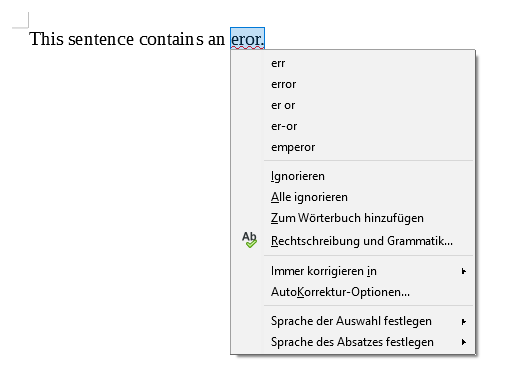
\includegraphics[width=\linewidth]{word_error}
  \caption{A subfigure}
  \label{fig:sub1}
\end{subfigure}%
\begin{subfigure}{.5\textwidth}
  \centering
  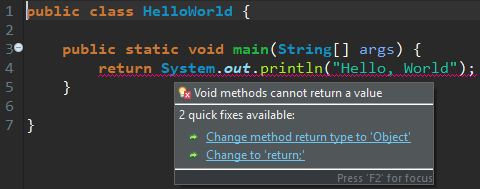
\includegraphics[width=\linewidth]{eclipse_error}
  \caption{A subfigure}
  \label{fig:sub2}
\end{subfigure}
\caption{A figure with two subfigures}
\label{fig:test}
\end{figure}

\subsection{Modern Approaches}


\section{Automatic Correction of Source Code}
